\documentclass[12pt,a4paper]{article}

\usepackage[T2A]{fontenc}
\usepackage[utf8]{inputenc}
\usepackage[russian]{babel}
\usepackage{amsmath,amssymb}
\usepackage{array}
\usepackage{booktabs}
\usepackage{geometry}
\usepackage{graphicx}
\usepackage{float}
\usepackage{listings}
\usepackage{caption}
\usepackage{enumitem}
\usepackage{indentfirst}
\usepackage{personal_data}
\usepackage{hhline}
\usepackage{tabularx}

\geometry{left=25mm,right=20mm,top=20mm,bottom=20mm}
\linespread{1.3}
\setlength{\parindent}{1.25cm}
\setlength{\parskip}{0.3em}

\lstset{
    basicstyle=\ttfamily\small,
    columns=fullflexible,
    frame=single,
    breaklines=true,
    keepspaces=true
}

\begin{document}

\begin{titlepage}
\center 

\normalsize \textbf{Липецкий государственный технический университет}\\

\vspace{1 cm}

\normalsize Институт компьютерных наук\\
\normalsize Кафедра прикладной математики и системного анализа\\

\vspace{6 cm}

\normalsize 	Отчет по лабораторной работе № \nomer_lr\\
по дисциплине <<\diszip >> \\
на тему <<\thema >>
\vspace{1 cm}


\vspace*{3 cm}

\normalsize
\begin{tabular}{b{4.75cm} p{1cm} c p{1cm} c}
Студент  	&   &  &  &  \student \\ \hhline{~~-~-} 

 	&  & \footnotesize \hspace{0.5cm} подпись, дата	\hspace{0.5cm} &  & \footnotesize  фамилия, инициалы \\ [-0.25cm]
Группа \underline{\group}  	&   &  &  &  \\ [0.4cm]
Руководитель  	&   &  &  &  \\
\centering{\dz}	&   &  &  & \dozent \\ \hhline{-~-~-} 
\footnotesize учёная степень, учёное звание	 	&  	& \footnotesize \hspace{0.5cm} подпись, дата	\hspace{0.5cm} &  & \footnotesize  фамилия, инициалы \\

 
\end{tabular} 



\vspace*{5cm}
\normalsize
\centering Липецк 2026 г.

\end{spacing}

\end{titlepage}

%\tableofcontents
\newpage

\section{Цель работы}

Изучить и практически реализовать алгоритмы прямого и обратного распространения ошибки для обучения многослойного перцептрона. Исследовать влияние архитектуры сети (число скрытых слоёв и нейронов) и скорости обучения на процесс минимизации функции потерь. Продемонстрировать необходимость нелинейных скрытых слоёв для решения задач, которые не являются
линейно разделимыми.

\section{Задание}

Необходимо реализовать обучение нейронной сети с использованием только алгоритмов прямого и обратного распространения ошибки (без использования готовых слоёв и оптимизаторов из библиотек глубокого обучения, таких как torch.nn или tensorflow.keras). Разрешается использовать библиотеки для работы с массивами (numpy) и для генерации данных (sklearn.datasets).

\section{Выбор датасета и подготовка данных}

В качестве датасета выбран \textbf{Two Moons} (\texttt{make\_moons}). Классы линейно неразделимы.

\begin{lstlisting}[caption={Исходный датасет}, label={lst:code_example}]
X, Y = make_moons(n_samples = 600, noise = 0.2, random_state=42)
X_train, X_test, Y_train, Y_test = train_test_split(X, Y, test_size = 0.3)
\end{lstlisting}

\begin{figure}[H]
    \centering
    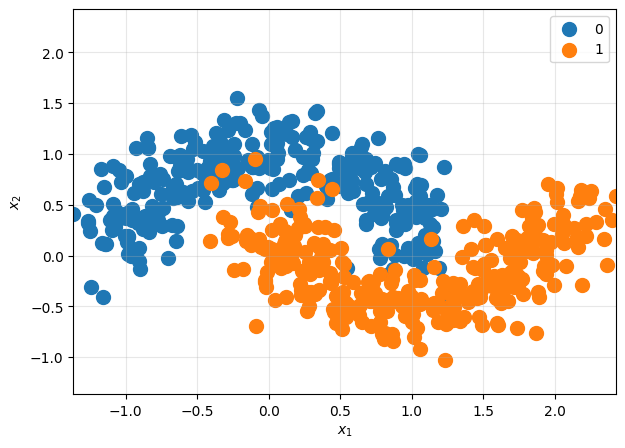
\includegraphics[scale=0.7]{dataset_visualization.png}
    \caption{Визуализация исходных данных}
    \label{fig:success}
\end{figure}

\section{Реализация нейронной сети и исследование архитектур}

\subsection{Реализация нейронной сети}

\begin{lstlisting}[caption={Математические функции}, label={lst:code_example}]
def tanh(x):
    return (math.exp(x) - math.exp(-x)) / (math.exp(x) + math.exp(-x))

def tanh_dif(x):
    return 1 - tanh(x) ** 2

def sigmoid(x):
    return 1 / (1 + math.exp(-x))

def sigmoid_dif(x):
    return sigmoid(x) * (1 - sigmoid(x))

def MSE(y_calc, y_real):
  total = 0
  for i in range(len(y_real)):
    total += (y_calc[i][0] - y_real[i]) ** 2
  return total / 2

def MSE_dif(y_calc, y_real):
  # sum = 0
  # for i in range(0, len(y_real)):
  #   sum += (y_calc[i] - y_real[i])
  # return [sum]
  return [y_calc[0] - y_real]
\end{lstlisting}

\begin{lstlisting}[caption={Класс нейрона}, label={lst:code_example}]
class Neuron:
  def __init__(self, num, activation = "sigmoid"):
    self.activation = activation
    self.weights = np.random.randn(num)
    self.bias = 0
    self.input = []
    self.output = 0
    self.dL_dw = []
    self.dL_db = 0

  def forward(self, input):
    self.input = input

    self.output = 0
    for i in range(len(self.input)):
      self.output += self.weights[i] * self.input[i]
    self.output += self.bias
    self.z = self.output
    self.output = (sigmoid(self.output) if self.activation == 'sigmoid' else tanh(self.output))

    return self.output

  def backward(self, dL_da):
    mul = dL_da * (sigmoid_dif(self.z) if self.activation == 'sigmoid' else tanh_dif(self.z))
    dL_dx = [mul * i for i in self.weights]
    self.dL_dw = [mul * i for i in self.input]
    self.dL_db = mul
    return dL_dx

  def update(self, learning_rate):
    self.weights = [self.weights[i] - learning_rate * self.dL_dw[i] for i in range(len(self.weights))]
    self.bias = self.bias - learning_rate * self.dL_db

\end{lstlisting}

\begin{lstlisting}[caption={Класс слоя}, label={lst:code_example}]
class Layer:
  def __init__(self, input_size, output_size, activation = "sigmoid"):
    self.neurons = [Neuron(input_size, activation) for i in range(output_size)]
    self.input_size = input_size
    self.output_size = output_size
    self.outputs = []

  def forward(self, input):
    self.outputs = []
    for neuron in self.neurons:
      self.outputs.append(neuron.forward(input))
    return self.outputs

  def backward(self, dL_da):
    dL_dx = [0] * self.input_size
    for i in range(self.output_size):
      dL_dx_cur = self.neurons[i].backward(dL_da[i])
      dL_dx = [dL_dx[j] + dL_dx_cur[j] for j in range(self.input_size)]
    return dL_dx

  def update(self, learning_rate):
    for neuron in self.neurons:
      neuron.update(learning_rate)

\end{lstlisting}

\begin{lstlisting}[caption={Класс сети}, label={lst:code_example}]
class Network:
  def __init__(self):
    self.layers = []
    self.loss = []

  def addLayer(self, layer):
    self.layers.append(layer)

  def forward(self, input):
    cur_input = input
    for layer in self.layers:
      cur_input = layer.forward(cur_input)
    return cur_input

  def backward(self, output):
    dL_da = MSE_dif(self.layers[-1].outputs, output)
    for i in range(len(self.layers) - 1, -1, -1):
      dL_da = self.layers[i].backward(dL_da)

  def predict(self, input):
    return self.forward(input)

  def update(self, learning_rate):
    for layer in self.layers:
      layer.update(learning_rate)

  def train(self, x_train, y_train, epoch = 100, learning_rate = 0.001):
    print('============================')
    for i in range(epoch):
      for x, y in zip(x_train, y_train):
        self.forward(x)
        self.backward(y)
        self.update(learning_rate)

      prediction = [self.forward(x_train[i]) for i in range(len(x_train))]
      loss = MSE([prediction[i] for i in range(len(prediction))], [y_train[i] for i in range(len(y_train))])
      self.loss.append(loss)
      if i % (epoch // 10) == 0:
        print(f"Epoch {i + 1}:")
        print(f"Loss: {loss}")
    print(f"Epoch {epoch}:")
    print(f"Loss: {loss}")
    print('============================')

  def get_loss(self):
    return self.loss

\end{lstlisting}

\subsection{Исследование архитектур}

\begin{lstlisting}[caption={Инициализация архитектур}, label={lst:code_example}]
models_layers = [[2, 1],
                 [2, 2, 1],
                 [2, 8, 1],
                 [2, 8, 8, 1]]

models = []
for m in models_layers:
  np.random.seed(42)
  network = Network()
  for i in range(1, len(m)):
    if i + 1 == len(m):
      network.addLayer(Layer(m[i - 1], m[i], 'sigmoid'))
    else:
      network.addLayer(Layer(m[i - 1], m[i], 'tanh'))
  models.append(network)
\end{lstlisting}

\begin{lstlisting}[caption={Обучение моделей}, label={lst:code_example}]
epoch = 5000
learning_rate = 0.01

fig, ax = plt.subplots(nrows=2, ncols=2, figsize=(8,8))
axes = ax.flatten()

for i in range(4):
  print(f"Model with layers {models_layers[i]}")
  models[i].train(X_train, Y_train, epoch = epoch, learning_rate = learning_rate)
  train_loss = models[i].get_loss()
\end{lstlisting}

\begin{figure}[H]
    \centering
    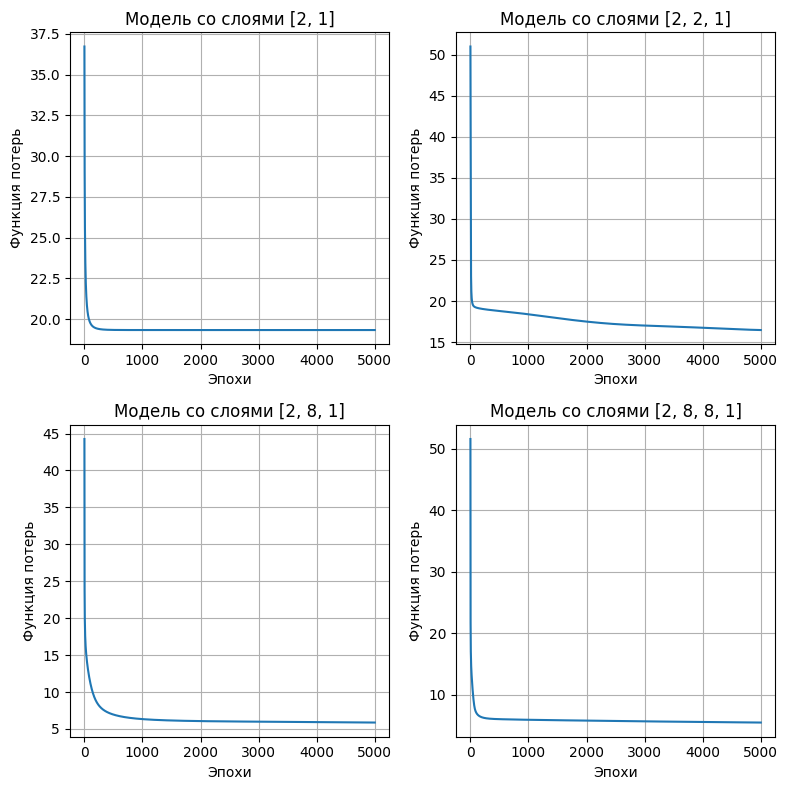
\includegraphics[scale=0.7]{2_2 loss.png}
    \caption{Графики функции потерь от эпох}
    \label{fig:success}
\end{figure}


\begin{table}
    \centering
    \begin{tabular}{|l|l|l|}
        \hline
        Модель           & Train & Test  \\ \hline
        {[}2, 1{]}       & 0.879 & 0.867 \\ \hline
        {[}2, 2, 1{]}    & 0.869 & 0.883 \\ \hline
        {[}2, 8, 1{]}    & 0.969 & 0.972 \\ \hline
        {[}2, 8, 8, 1{]} & 0.971 & 0.961 \\ \hline
    \end{tabular}
    \caption{Точность моделей}
    \label{tab:placeholder}
\end{table}

\begin{figure}[H]
    \centering
    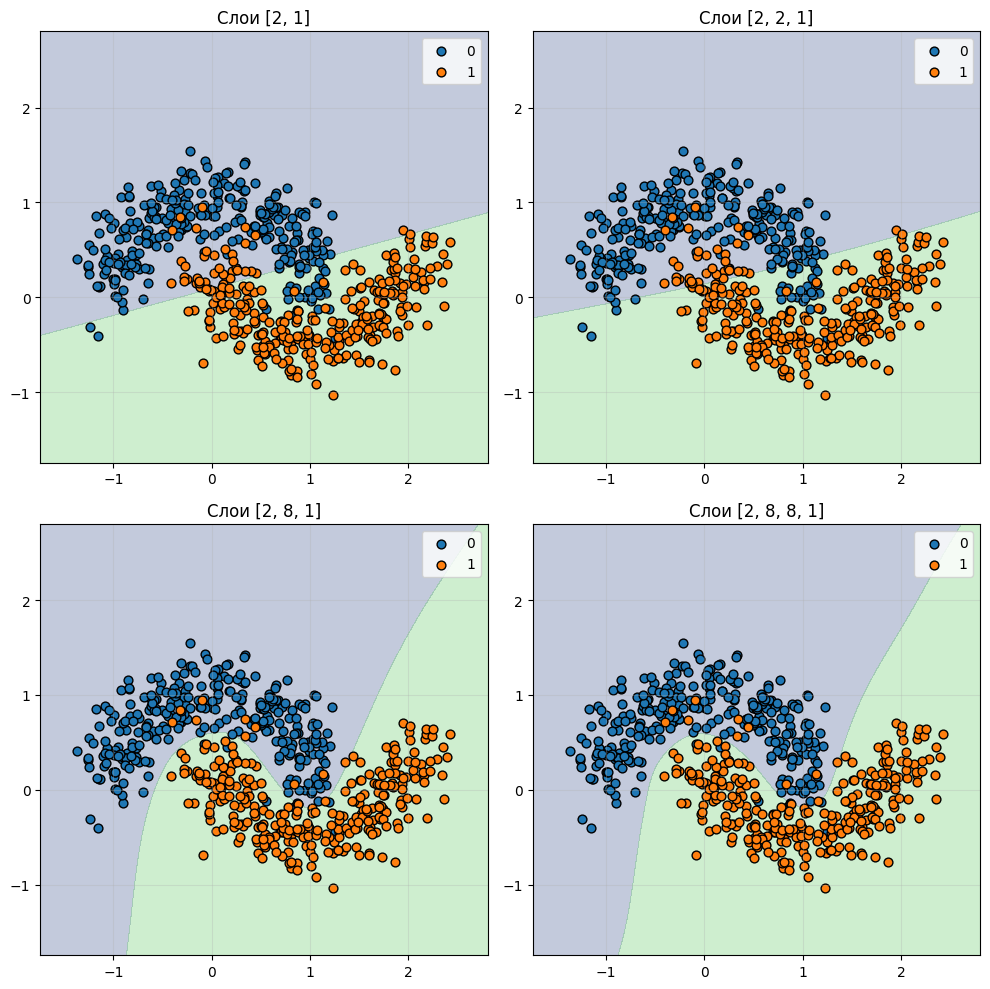
\includegraphics[scale=0.7]{resh_gran.png}
    \caption{Визуализация решающих границ}
    \label{fig:success}
\end{figure}

\section{Исследование скорости обучения (learning rate)}

Лучшая модель со слоями [2, 8, 1]. Её точность сравнима с точностью модели [2, 8, 8, 1], но эта (вторая) модель имеет большее число слоёв, нейронов и связей, она будет медленее.

Сравним обучение модели [2, 8, 1] с learning rate: $r \in \{0.001,0.01,0.1,1.0\}$.

\begin{figure}[H]
    \centering
    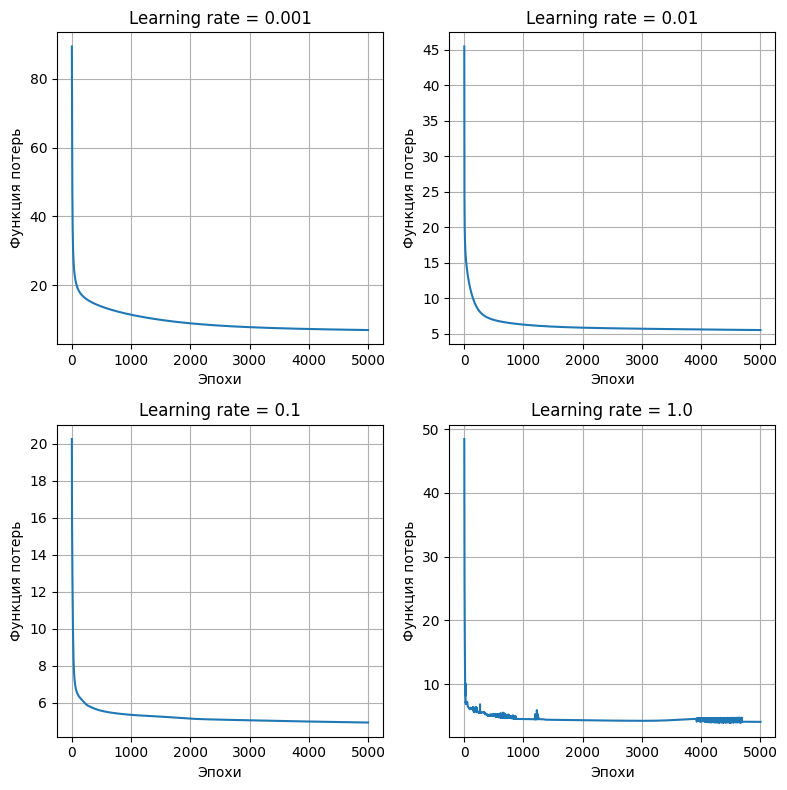
\includegraphics[scale=0.7]{loss for learning_rate.png}
    \caption{Графики функций потерь для моделей с разными learning rate}
    \label{fig:success}
\end{figure}

% \begin{table}[H]
%     \centering
%     \begin{tabular}{l c c c c r}
%         \hline
%         \(r\) & Эпоха с Loss \(< 5\) & Loss на эпохе 500 & Loss на эпохе 1000 & Loss на эпохе 2000 & Loss на эпохе 5000 \\
%         \hline
%         0.001 & -- & \(\sim\)13.8 & \(\sim\)11.4 & \(\sim\)8.9 & \(\sim\)7.07 \\
%         0.01  & -- & \(\sim\)6.97 & \(\sim\)6.3  & \(\sim\)5.88 & \(\sim\)5.54 \\
%         0.1   & \(\sim\)3500 & \(\sim\)5.56 & \(\sim\)5.3 & \(\sim\)5.1 & \(\sim\)4.93 \\
%         1.0   & \(\sim\)500  & \(\sim\)5.05 & \(\sim\)4.5 & \(\sim\)4.3 & \(\sim\)4.39 \\
%         \hline
%     \end{tabular}
%     \caption{Сравнение скоростей обучения}
%     \label{tab:placeholder}
% \end{table}

\begin{table}[H]
    \centering
    \small
    \setlength{\tabcolsep}{4pt}
    \begin{tabularx}{\textwidth}{l *{5}{>{\centering\arraybackslash}X}}
        \hline
        \(r\) & Эпоха с & Loss на & Loss на & Loss на & Loss на \\
              & Loss \(<5\) & эпохе 500 & эпохе 1000 & эпохе 2000 & эпохе 5000 \\
        \hline
        0.001 & --         & \(\sim\)13.8 & \(\sim\)11.4 & \(\sim\)8.9  & \(\sim\)7.07 \\
        0.01  & --         & \(\sim\)6.97 & \(\sim\)6.3  & \(\sim\)5.88 & \(\sim\)5.54 \\
        0.1   & \(\sim\)3500 & \(\sim\)5.56 & \(\sim\)5.3  & \(\sim\)5.1  & \(\sim\)4.93 \\
        1.0   & \(\sim\)500  & \(\sim\)5.05 & \(\sim\)4.5  & \(\sim\)4.3  & \(\sim\)4.39 \\
        \hline
    \end{tabularx}
    \caption{Сравнение скоростей обучения}
    \label{tab:placeholder}
\end{table}

При увеличении learning rate скорость выхода на плато возрастает: r=0.1 и r=1.0 достигают плато за первые ~500 эпох, r=0.01 — примерно к 1500-й, а r=0.001 подходит к нему лишь к концу 5000 эпох. Однако, при learning rate=1.0 можно заметить, что функция потерь теряет монотонность, ее значения (а значит и график) начинают с определённого момента иногда колебаться, из-за чего график получается не гладким, а со скачками.

\section{Выводы и анализ результатов}

Линейная модель (без скрытых слоёв) не справляется с линейно неразделимыми данными:
\begin{enumerate}
    \item Из графика с решающей границей мы видим, что набор данных не линейный и его невозможно разделить на две группы одной прямой линий;
    \item В сравнении точности линейной модели с другими видно, что она уступает другим и и на 10 п.п. на тестовой выборке.
\end{enumerate}


Увеличение числа нейронов и слоёв повышает выразительную способность сети. С увеличением нейронов слоёв мы видим:
\begin{enumerate}
    \item На графиках решающих границ, эти границы уже не просто прямые, но кривые, которые лучше разделяю области данных на группы;
    \item Точности моделей [2, 8, 1] и [2, 8, 8, 1] лучше моделей [2, 1] и [2, 2, 1].
\end{enumerate}


Почему для данной задачи необходима нелинейная функция активации? При обучении моделей используется алгоритм обратного распространения и идея градиентного спуска. Градиент — это вектор частных производных, следовательно, для его вычисления необходима дифференцируемость. При этом функция должна также иммитировать ступенчатую функцию (функция Хевисайда не является дифференцируемой).
\\

Вывод о влиянии скорости обучения на сходимость градиентного спуска. Малые r дают стабильное, но медленное обучение; большие — быстрое, но менее устойчивое.

\end{document}